
\section{Introduction}

For this assessment, I choose to used IntelliJ IDEA to run my test coverage, a test coverage give the possibility to figure out which part of the code is cover by my unit test. IntelliJ is pre-installed with it's on test/code coverage tool. The plugin is available by default/ Moreover, to launch our first coverage, we just need to click on the appropriate button, which is just under the button to compile the project.

\section{Unit Test}

I choose to handle my Unit test with JUnit. The latter is not directly installed, but this can be done in a few simple actions by navigating into the menus. The JUnit library is available within the Maven repository.


\subsection{Configure the project for Unit Test:}


It is not a mandatory part, however, as it is a great practice to create a folder dedicated to Unit Test, I started with this step. To do it we need to precise to Iteliji the location of our test folder. We can do it by going to the "Project Structure Setting" and select a folder of our choice.

\subsection{Create a first Unit Test:}

By pressing Alt+Enter on any class, we can create a first JUnit test and automatically select the methods we are interested in. Then, a new pre-filled script is built in the Test folder. Once I am in my file, I can create any analysis I want, method per method. One of the good things here is the possibility to test any of them one by one. Without running all the class. Good point, however, this impel us to declare a new instance of the class to test in each method. What is not very convenient.

From a design point of view, the user experience is very nice, a green bar appears to the bottom to directly indicate that 100\% tests are confirmed. It is further what we are looking for. Moreover, If somehow we forgot to add methods to the test class, we can quickly add it by pressing alt+insert. This, open a new menu where we can select the desired method to insert.

Once we are happy with our first test methods, we can run a test using the test coverage tool. This one can be directly accessible by clicking slightly below the run method.


\begin{figure}[H]
  \centering
  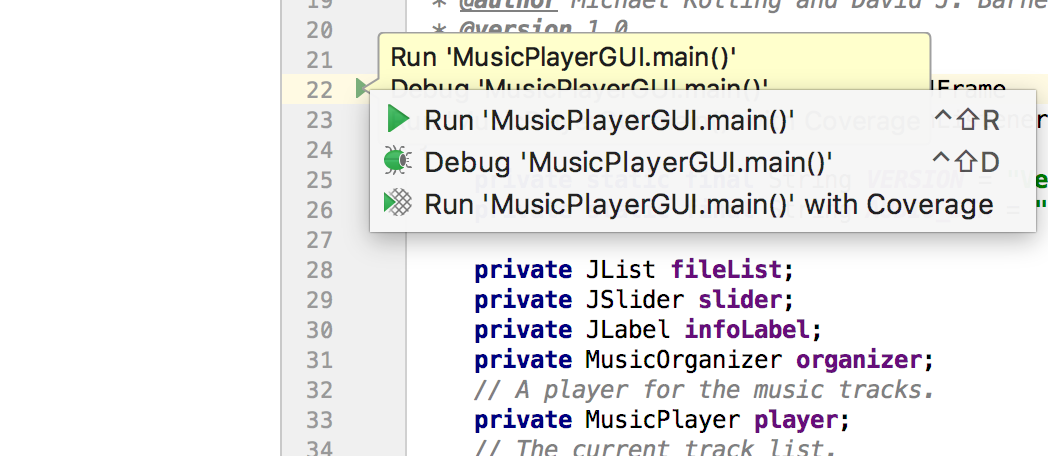
\includegraphics[width=8cm]{body/s1.png}
  \caption{Run a test coverage}
\end{figure}

\section{Test coverage}

To check the result of the test coverage we got a direct access on the right of the window to a summary table showing some useful pieces of information. First, a list indicates whether a class is covered by some test or not. Then, the percentage of methods analyze and the portion of lines cover. In order to get more details about which method and which line are tested, all we need to dot is to click on the corresponding class. Then, above each line, a color label (red or green) is added in order to distinguish both class (tested or not).

Note about the color: Is possible to edit the coverage tools to changes colors, which a perfect features, showing once again the ambition from IntelliJ to propose good technical services as well as a good user experience.

\subsubsection{Advanced settings}

If we want to go further, it is possible to customise the coverage tool. Indeed, instead of running a Test class, we can do the same thing for a Pattern or a Category. Moreover, we can choose the way the test code is executed by running each task in a separate process. One of my favorites features is the "Test Cover export".  Indeed its give the possibility to export the result of the coverage in a separate document. In this case, in HTML. This report is a breakdown of all method and classes. We can use it is to work with a team and to share/save the state of a project at a given time.

\begin{figure}[H]
  \centering
  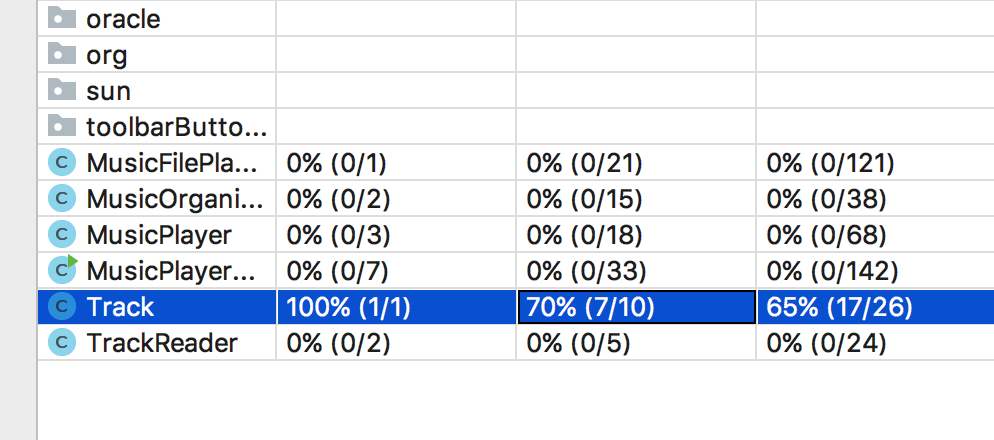
\includegraphics[width=8cm]{body/s2.png}
  \caption{Result of test coverage - Percentages}
\end{figure}

\begin{figure}[H]
  \centering
  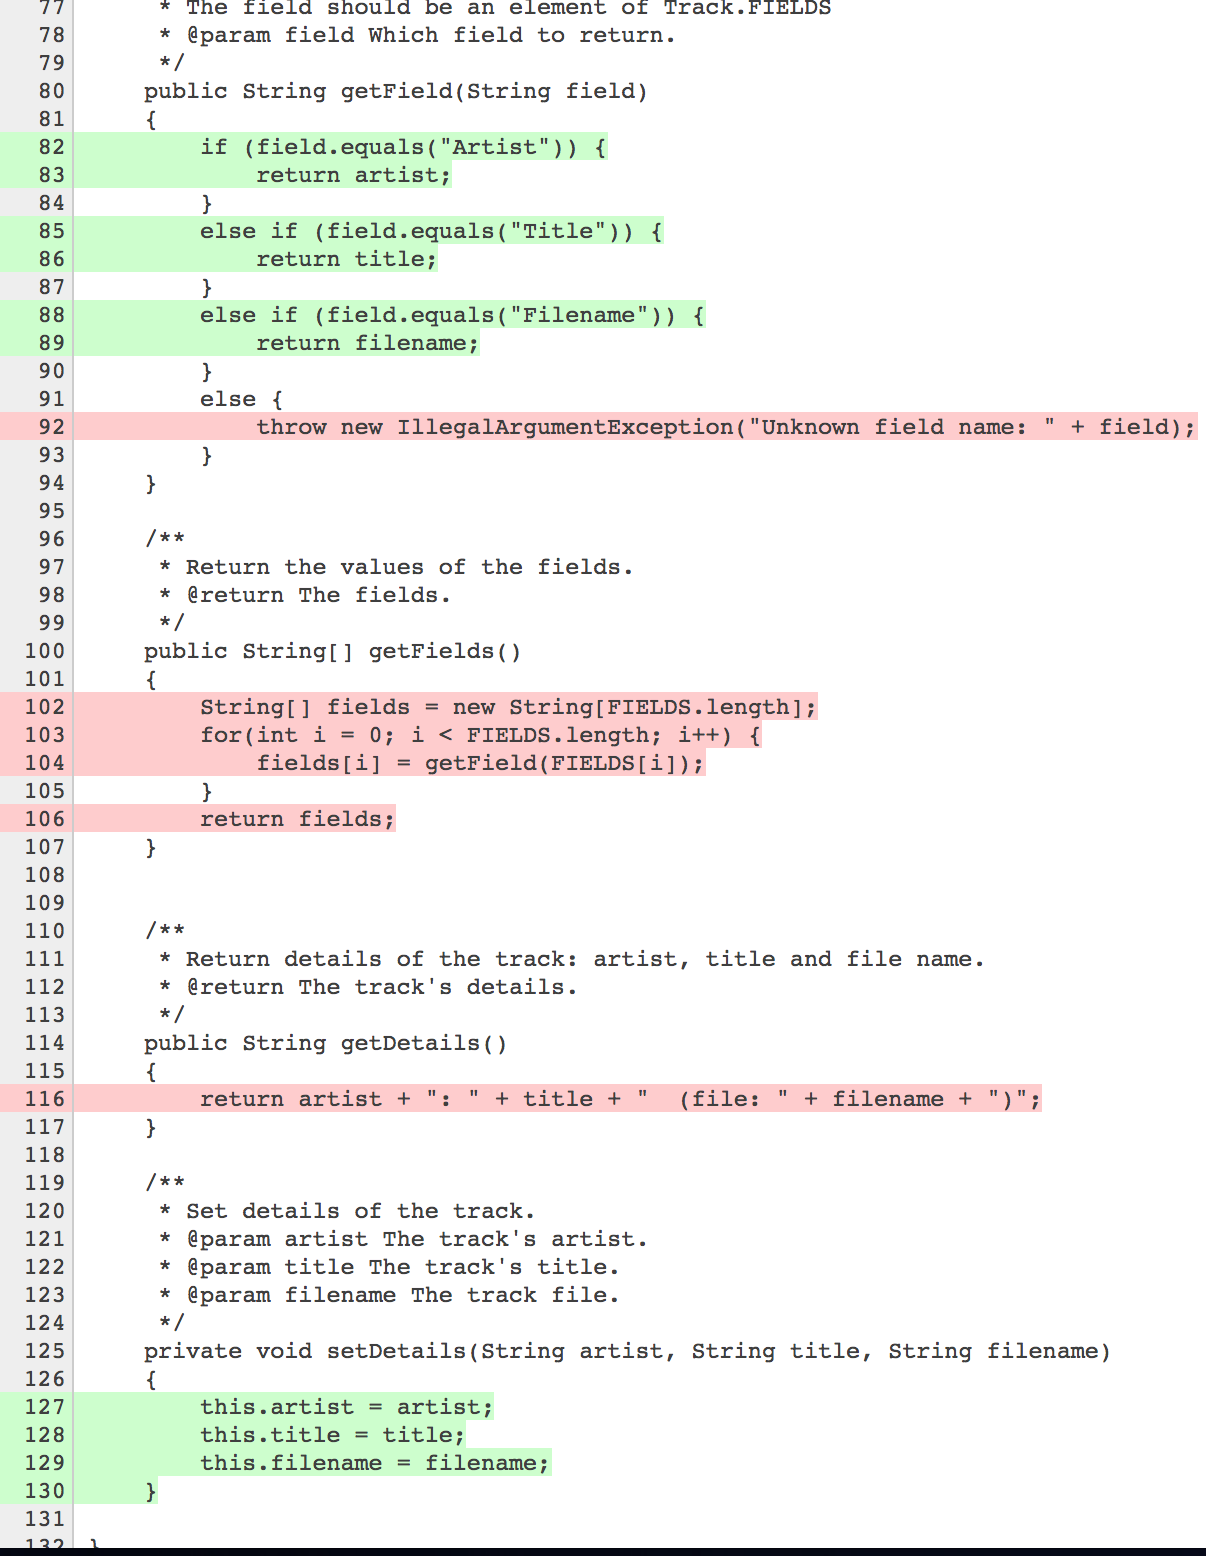
\includegraphics[width=8cm]{body/s3.png}
  \caption{Result of test coverage - Class}
\end{figure}
